\documentclass[10pt]{beamer}

\usepackage{ifplatform}
\usepackage{verbatim}
\usepackage{graphicx}
\usepackage{epstopdf}
\graphicspath{{../figures/}}
\epstopdfsetup{outdir=./converted/}
\usepackage{float}
\usepackage{amsmath}
\usepackage{amssymb}
\usefonttheme[onlymath]{serif}
% SVG Package Options
\usepackage{svg}
\svgpath{ {../figures/} }
\svgsetup{inkscapeformat=pdf} % pdf/eps/ps/png
\svgsetup{inkscapelatex=true} % true/false
\svgsetup{inkscapearea=drawing} % drawing/page
\ifwindows
\setsvg{inkscapeexe={"C:/Program Files/Inkscape/inkscape.com"}}
\fi
%\svgsetup{inkscapedpi=300} % <integer>
\svgsetup{inkscapepath=./converted/}
%svgdir/svgpath
%   The PDF/EPS/PS/PNG graphic files as well as LATEX files generated by Inkscape
%   will be located in same directory as corresponding SVG file.
%svgsubdir/svgsubpath
% Within folder of encountered SVG file, all exported files will be located in a
% subfolder named svg-inkscape/.
%basedir/basepath/jobdir/jobpath
% All exported files will be located in current working directory.
%basesubdir/basesubpath/jobsubdir/jobsubpath
% A subfolder named svg-inkscape/ within current working directory will be used
% for files generated by Inkscape.
%/path/to/somewhere/
% It is also possible to give a custom path, either relative to current working directory (./relative/path/) or as an absolute path.
\ifpdftex
\pdfsuppresswarningpagegroup=1

\usetheme{metropolis}
\usepackage{appendixnumberbeamer}
\usepackage{booktabs}
\usepackage[scale=2]{ccicons}
\usepackage{pgfplots}
\usepgfplotslibrary{dateplot}
\usepackage{xspace}
\newcommand{\themename}{\textbf{\textsc{metropolis}}\xspace}

\setbeamertemplate{frametitle continuation}{}
\setbeamertemplate{footline}{}

\begin{document}

\title{Modelling and Control of WEDM Process for Cutting of Si-Ingots}
\author{Akshay Khadse \\ Roll No. 153079011 \\ Guide: Prof. S. V. Kulkarni}
\date{\today}
\maketitle

\begin{frame}{Table of contents}
  \setbeamertemplate{section in toc}[sections numbered]
  \tableofcontents[hideallsubsections]
\end{frame}

\section{Introduction}
\begin{frame}{Introduction}
  \begin{itemize}
    \item Solar energy: \alert{prominent source} of renewable energy
    \item Extracting silicon wafers accounts for \alert{20\%} of total energy consumption throughout process \cite{del09}
    \item Popular methods for silicon cutting: \\ i) Wire loose slurry method \\ ii) Diamond saw cutting method
    \item Abrasive nature - lead to \alert{micro-fractures} up to 20 $\mu$m deep
    \item Wafer size gets limited to \alert{180 $\mu$m} \cite{sopori13}
    \item 50\% of ingot material is lost as \alert{kerf losses} \cite{joshi10}
    \item \alert{Contamination} of wafers due to slurry, etc. \cite{moeller2015}
  \end{itemize}
\end{frame}

\begin{frame}[allowframebreaks]{Wire Electro-Discharge Machining}
  \begin{figure}
    \centering
    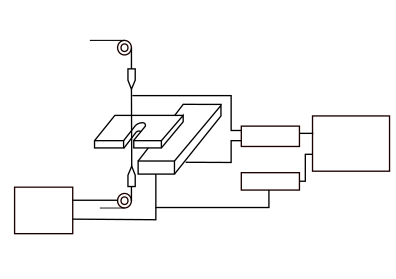
\includegraphics[width=0.9\textwidth]{wedm-diag}
    \caption{Diagrammatic representation of WEDM}
    \label{fig:lit-1}
  \end{figure}
  \framebreak
  \begin{itemize}
    \item \alert{Non contact} micro-drilling process
    \item Cuts free form contours from large solid metal workpieces
    \item \alert{No force exerted} on workpiece \textendash{} Thinner wires can be used
    \item \alert{Reduced kerf width} \cite{dongre2015multi} \\ 250 $\mu$m \textendash{} Abrasive saw cutting \\ 50 $\mu$m \textendash{} WEDM
    \item Net material saving of 200 \textendash{} 300\% \cite{dongre2015multi}
    \item WEDM: A promising alternative for silicon wafer manufacturing
    \item Goal: Optimise WEDM process for silicon wafers
  \end{itemize}

  \framebreak
  \begin{itemize}
    \item WEDM is not as well established for silicon
    \item Electrical characterisation of \alert{metal-semiconductor-dielectric} sparks
    \item \alert{VI characteristics} of silicon are very \alert{different} from that of steel \cite{kane2017aps}
    \item Settings on commercial WEDM machines are only \alert{applicable for steel} \cite{levy1990wed}
    \item Available machines have discrete setting ranges
    \item Indigenously designed power supply required
    \item Completed: Design, modelling and control of such power supply 
  \end{itemize}
\end{frame}

\section{Literature Survey}

\begin{frame}[allowframebreaks]{Research areas}
\begin{table}
  \begin{tabular}{p{3.5cm} p{7cm}}
    \hline
    \multicolumn{2}{l}{Process Modelling} \\
    \hline
    Spur and Sch{\"o}nbeck \cite{spur1993anode} & Influence of \alert{work-piece material} and \alert{pulse type}\\
    Han et al. \cite{han2002high} & Simulated \alert{discharge phenomena} of WEDM, developed adaptive control system\\
    \hline
    \multicolumn{2}{l}{Fuzzy Control Systems} \\
    \hline
    Kinoshita et al. \cite{kinoshita1976study} & Investigated effects of \alert{wire feed rate, winding speed, tension and electrical parameters}\\
    De Bruyn et al. \cite{de1982has} & Classified EDM pulses as \alert{open, spark, arc, off or, short} on basis of ignition delay\\
    \hline
    \multicolumn{2}{l}{Wire Breakage Avoidance} \\
    \hline
    Kinoshita et al. \cite{kinoshita1982control} & Rapid rise in \alert{pulse frequency} of voltage before \alert{wire breakage}, developed a monitoring system that switches off pulse generator\\
    N. Kinoshita, M. Fukui, and G. Gamo \cite{kunieda1990line} & Increase in \alert{localised temperature} at certain points of wire leads to its breakage, system for \alert{detection of spark location}
  \end{tabular}
\end{table}
\begin{table}
  \begin{tabular}{p{3.5cm} p{7cm}}
    \hline
    \multicolumn{2}{l}{Wire lag and wire vibration} \\
    \hline
    Duaw and Beltrami \cite{dauw1994high} & Used \alert{optical sensor} for monitoring and control of wire position \\
    N. Mohri et al. \cite{mohri1998system} & Several mathematical models \textendash{} transient response of \alert{wire vibration} \textendash{} force acting on tool\\
    \hline
    \multicolumn{2}{l}{Adaptive control systems} \\
    \hline
    Kinoshita et al. \cite{kinoshita1982control} & Change in \alert{work-piece thickness} \textendash{} increase in wire thermal density\\
    Rajurkar et al. \cite{rajurkar1997wedm} & Adaptive control \& multiple input model \textendash{} monitors \& controls \alert{sparking frequency} according to on-line identified \alert{work-piece height}\\
    \hline
  \end{tabular}
\end{table}
\end{frame}

\section{Power Supply Design}
\begin{frame}[allowframebreaks]{Working Principle}
\visible<1>{
  \begin{figure}
    \centering
    \includesvg[width=0.9\textwidth]{rep-diag-master}
    \caption{Representative diagram of ideal WEDM power supply}
    \label{fig:working-1}
  \end{figure}
}
\visible<2>{
  \begin{figure}
    \centering
    \includesvg[height=3.5cm]{rep-diag-1}
  \end{figure}
  \vspace{-1.3cm}
  \begin{figure}
    \centering
    \includesvg[height=5cm]{working-wf-1}
  \end{figure}
}
\visible<3>{
  \begin{figure}
    \centering
    \includesvg[height=3.5cm]{rep-diag-3}
  \end{figure}
  \vspace{-1.3cm}
  \begin{figure}
    \centering
    \includesvg[height=5cm]{working-wf-2}
  \end{figure}
}
\visible<4>{
  \begin{figure}
    \centering
    \includesvg[height=3.5cm]{rep-diag-3}
  \end{figure}
  \vspace{-1.3cm}
  \begin{figure}
    \centering
    \includesvg[height=5cm]{working-wf-3}
  \end{figure}
}
\visible<5>{
  \begin{figure}
    \centering
    \includesvg[height=3.5cm]{rep-diag-4}
  \end{figure}
  \vspace{-1.3cm}
  \begin{figure}
    \centering
    \includesvg[height=5cm]{working-wf-4}
  \end{figure}
}
\visible<6>{
  \begin{figure}
    \centering
    \includesvg[height=3.5cm]{rep-diag-4}
  \end{figure}
  \vspace{-1.3cm}
  \begin{figure}
    \centering
    \includesvg[height=5cm]{working-wf-5}
  \end{figure}
  \vspace{-0.35cm}
}
\end{frame}

\begin{frame}{Converter Topology}
  \begin{figure}
    \centering
    \includesvg[width=0.9\textwidth]{conv-top-master}
    \caption{Converter topology for WEDM power supply \cite{tastekin2009novel}}
    \label{fig:working-3}
  \end{figure}
\end{frame}

\section{Converter Modelling}

\begin{frame}{Voltage Source Modelling}
  \begin{figure}
    \centering
    \includesvg[width=0.7\textwidth]{buck-2}
    \caption{Simplified circuit of two quadrant converter used as voltage source}
    \label{fig:working-4}
  \end{figure}

\end{frame}

\begin{frame}{Voltage Source Modelling}
\begin{enumerate}
\item State variables: $i_{L_2} \rightarrow x_1$, $v_{c_2} \rightarrow x_2$
\item Switch ON state $\rightarrow$ State equations (E1)
\item Switch OFF state $\rightarrow$ State equations (E2)
\item Time averaging (E1) and (E2)
  \begin{equation}
    \begin{split}
      \dot{x} &= [dA_1+(1-d)A_2]x + [dB_1 + (1-d)B_2]V_d\\
      V_o &= [dC_1+(1-d)C_2]x
    \end{split}
    \label{eq:mod14}
  \end{equation}
\item Small signal perturbation in $d$
\item Get $\dfrac{\hat{v}_o(s)}{\hat{d}(s)}$
\end{enumerate}
\end{frame}

\begin{frame}{Voltage Source Modelling}
  \begin{figure}
    \centering
    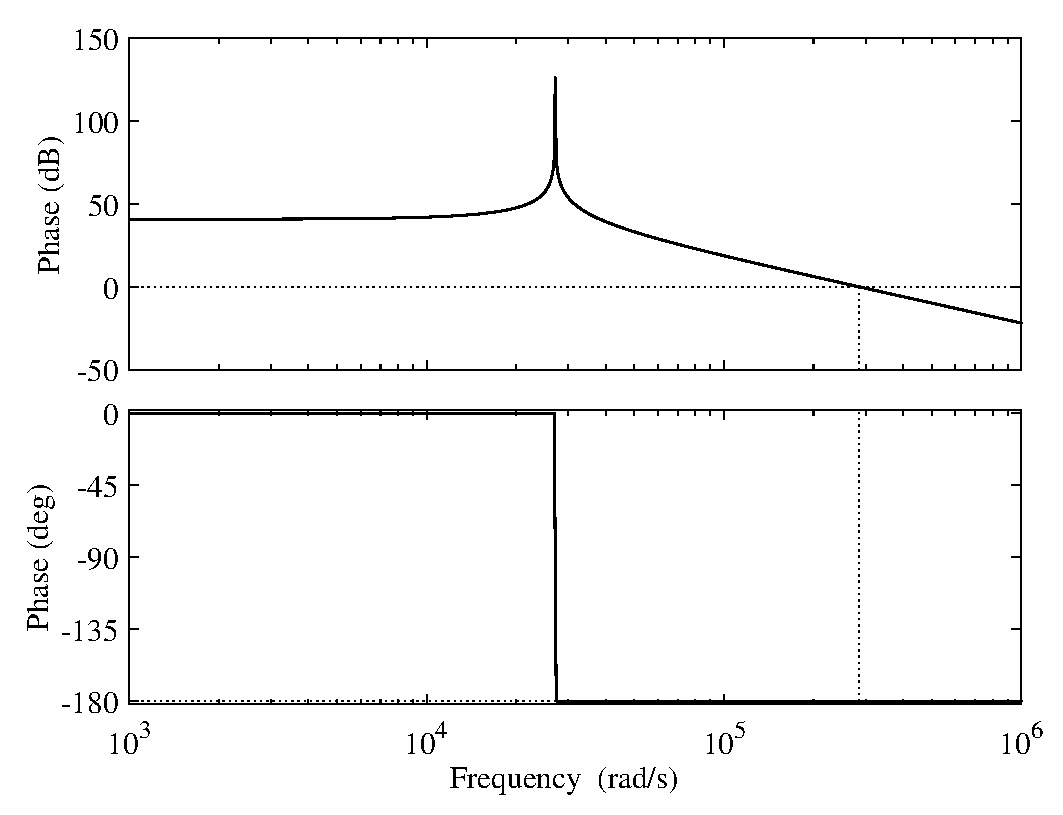
\includegraphics[width=0.8\textwidth]{uncompensated-vs}
    \caption{Bode plot of uncompensated transfer function of voltage source; \hspace{1cm} Gm = $\infty$,  Pm = 0.0166$^\circ$ (at 2.85e+05 rad/s)}
    \label{fig:uncomp-vs}
  \end{figure}
\end{frame}

\begin{frame}{Current Source Modelling}
  \begin{figure}
    \centering
    \includesvg[width=0.7\textwidth]{buck-1-master}
    \caption{Simplified circuit of single quadrant converter used as current source}
    \label{fig:working-5}
  \end{figure}
  \vspace{-0.5cm}
  \begin{enumerate}
\item State variable: $i_{L_1} \rightarrow x$
\item Same steps as voltage source
  \begin{equation}
    \begin{split}
      \dot{x} &= [dA_1+(1-d)A_2]x + [dB_1 + (1-d)B_2]V_d\\
      I_o &= [dC_1+(1-d)C_2]x
    \end{split}
    \label{eq:mod14}
  \end{equation}
\item Small signal perturbation in $d$
\item Get $\dfrac{\hat{i}_o(s)}{\hat{d}(s)}$
\end{enumerate}
\end{frame}

\begin{frame}{Current Source Modelling}
  \begin{figure}
    \centering
    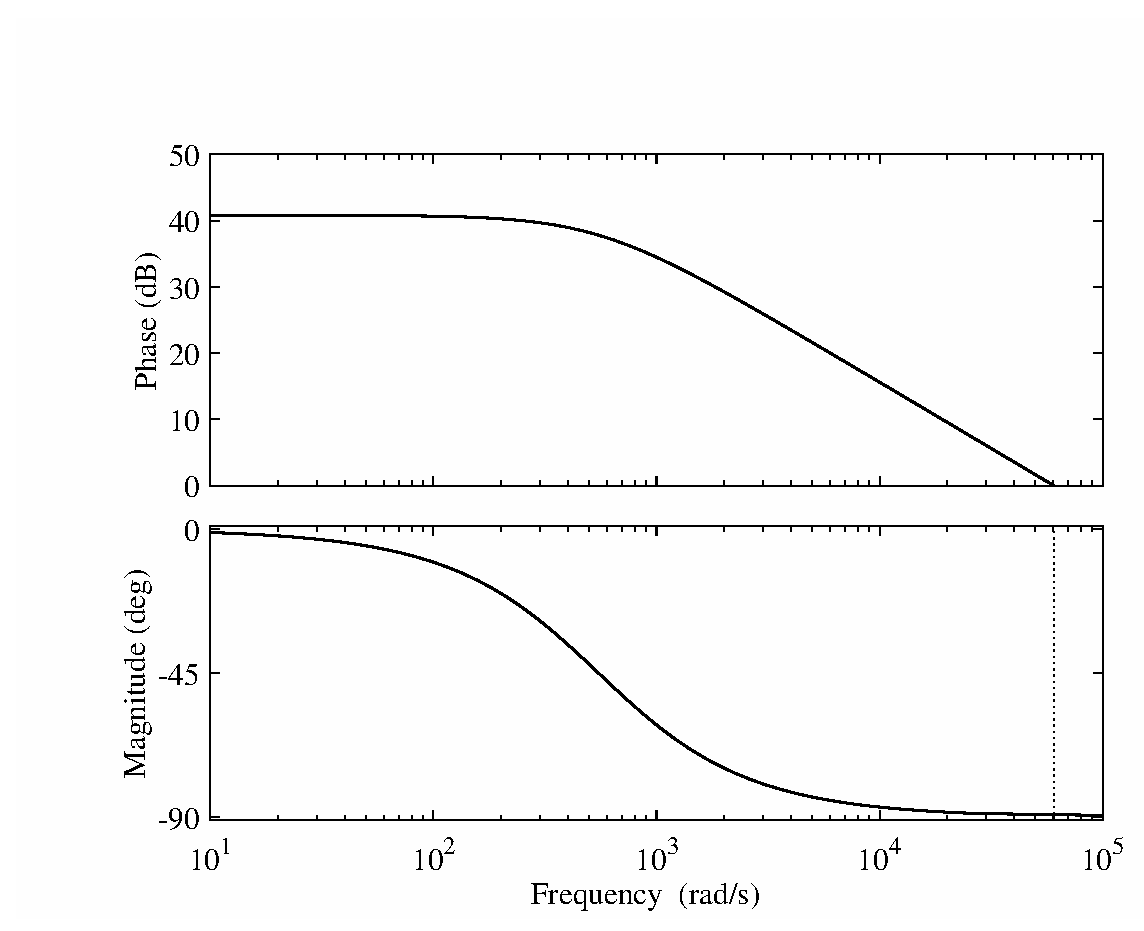
\includegraphics[width=0.8\textwidth]{uncompensated-cs}
    \caption{Bode plot of uncompensated current source transfer function; \hspace{1cm} Gm = $\infty$,  Pm = 90.5$^\circ$ (at 6.05e+04 rad/s)}
    \label{fig:uncomp-cs}
  \end{figure}
\end{frame}

\section{Controller Design}
\begin{frame}{Direct Duty Ratio Control}

\begin{figure}
  \centering
  \includesvg[width=0.8\textwidth]{direct-duty}
  \caption{Direct duty ratio control of single quadrant converter}
  \label{fig:dirduty-1}
\end{figure}
\end{frame}

\begin{frame}{Direct Duty Ratio Control}
\begin{enumerate}
\item Design lead compensator s.t.
\begin{enumerate}
\item Gain crossover freq \textendash{} high, less than $F_s$
\item Phase margin between 45$^\circ$ to 60 $^\circ$
\end{enumerate}
\item Check steady state error
\item Design lag compensator s.t.
\begin{enumerate}
\item Max phase lag frequency $<<$ gain crossover frequency
\item Sufficient gain is added at lower frequency
\end{enumerate}
\item Balance loop gain at gain crossover
\end{enumerate}

\end{frame}

\begin{frame}{Direct Duty Ratio Control}
  \begin{figure}
    \centering
    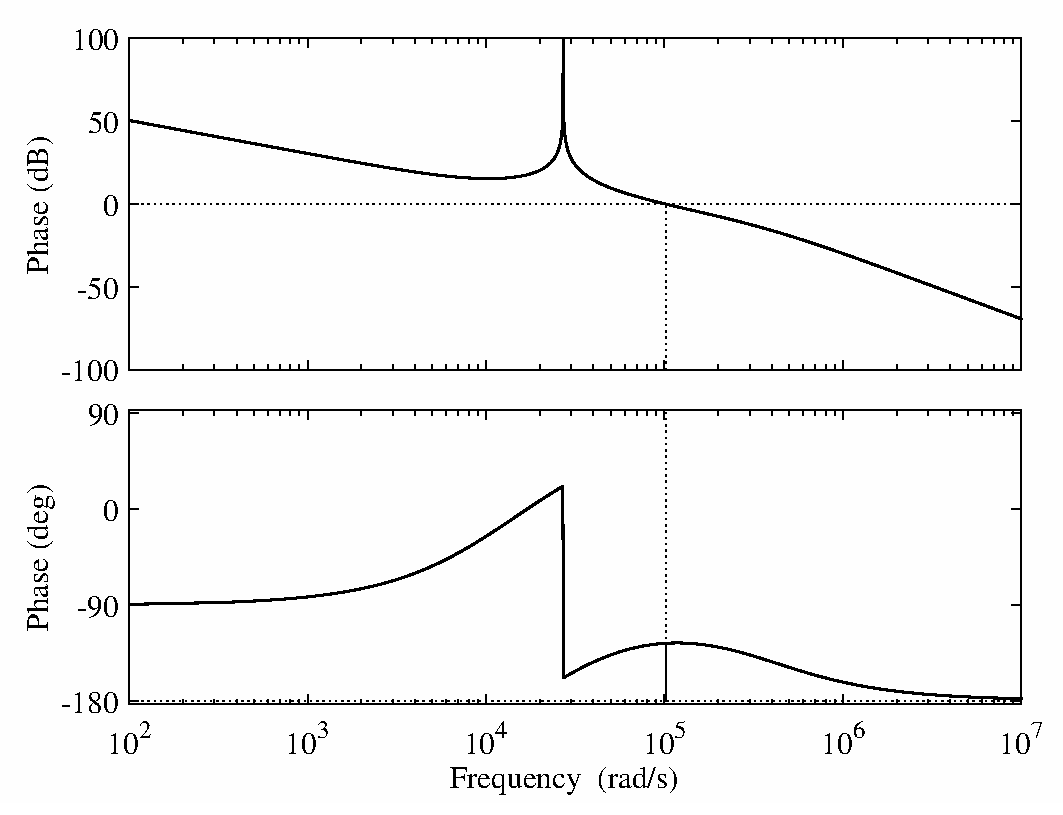
\includegraphics[width=0.8\textwidth]{compensated-vs}
    \caption{Bode plot of compensated transfer function of voltage source \hspace{1cm} Gm = $\infty$,  Pm = 54.3$^\circ$ (at 1.02e+05 rad/s)}
    \label{fig:comp-vs}
  \end{figure}
\end{frame}

\begin{frame}{Result}
  \begin{figure}
    \centering
    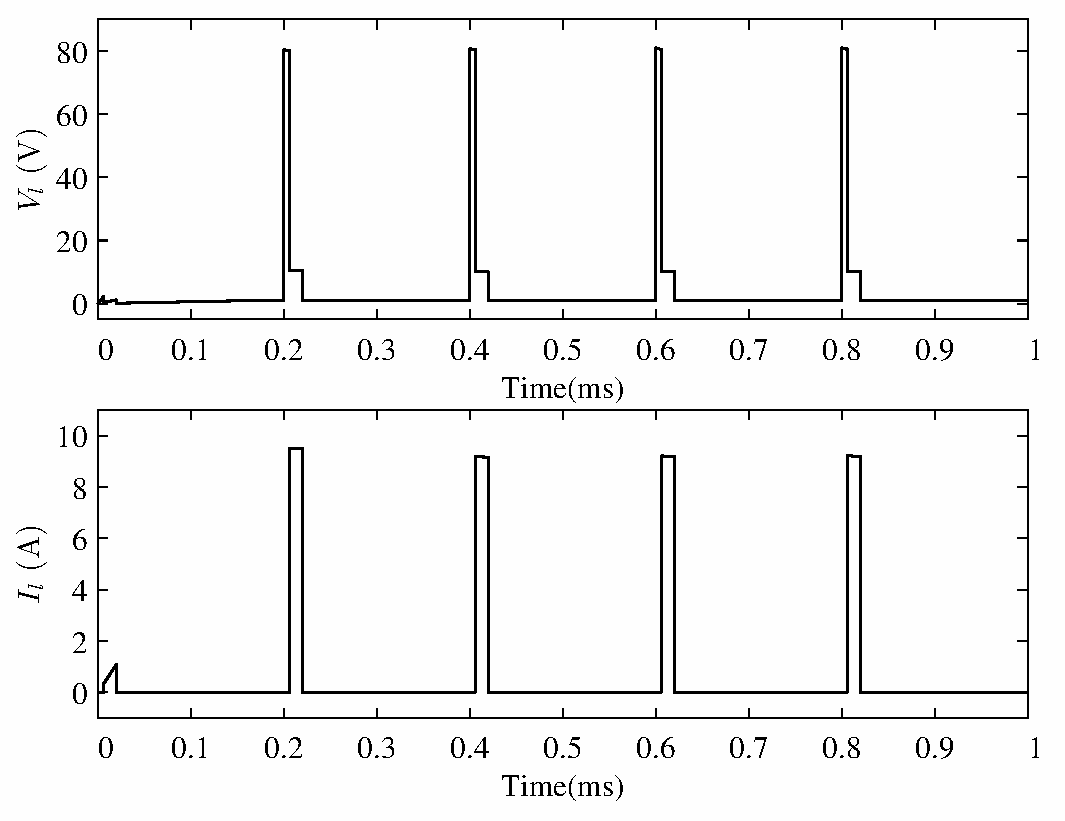
\includegraphics[width=0.8\textwidth]{load_comp}
    \caption{Load voltage and current - direct duty ratio control}
    \label{fig:1b}
  \end{figure}
\end{frame}

\begin{frame}{Alternatives}
\textbf{Disadvantages of direct duty ratio control}
\begin{itemize}
\item Separate protection circuit required
\item Current sensors not utilized for control
\end{itemize}
\textbf{Advantages of current mode control}
\begin{itemize}
\item Inherent protection against over current
\item First order model for voltage control
\end{itemize}
\textbf{Disadvantages of current mode control}
\begin{itemize}
\item Susceptible to noise
\end{itemize}
\end{frame}

\begin{frame}{Current Mode Control}
\begin{columns}
\begin{column}{0.5\textwidth}
  \begin{figure}
    \centering
    \includesvg[width=1.1\textwidth]{current-mode-minimal-master}
    \caption{Current mode control of single quadrant converter}
    \label{fig:16}
  \end{figure}
    \begin{equation}
    \dfrac{m_2}{m_1} = \dfrac{d}{1-d}
    \label{eq:4}
  \end{equation}
\end{column}
\begin{column}{0.5\textwidth}
  \begin{figure}
    \centering
    \includesvg[width=\textwidth]{switch-current}
    \vspace{-0.85cm}
    \caption{Switch current in current mode control}
    \label{fig:17}
  \end{figure}
  \vspace*{-0.8cm}
  \begin{figure}
    \centering
    \includesvg[width=\textwidth]{inductor-current}
    \vspace{-0.9cm}
    \caption{Inductor current in current mode control}
    \label{fig:18}
  \end{figure}
\end{column}
\end{columns}

\end{frame}

\begin{frame}{Duty $>$ 0.5}
 \vspace{-0.2cm}
  \begin{figure}
    \centering
    \includesvg[width=0.6\textwidth]{wf-no-ramp}
    \vspace{-0.4cm}
    \caption{Inductor current in presence of disturbance}
    \label{fig:19}
  \end{figure}
  \vspace{-0.5cm}
  \begin{figure}
    \centering
    \includesvg[width=0.6\textwidth]{wf-ramp}
    \vspace{-0.4cm}
    \caption{Inductor current with artificial ramp in presence of disturbance}
    \label{fig:22}
  \end{figure}

\end{frame}

\begin{frame}{Voltage control using current mode control}
  \begin{figure}
    \centering
    \includesvg[width=0.65\textwidth]{current-mode-voltage-control}
    \caption{Controlled voltage source using current mode control}
    \label{fig:24}
  \end{figure}
\end{frame}

\begin{frame}{Modelling of voltage source}
\metroset{block=fill}
\begin{block}{Assumption}
  Current mode controller operates ideally i.e average inductor current $i_L$ to be identical to control $i_c$
\end{block}
\begin{figure}
  \centering
  \includesvg[width=0.6\textwidth]{modelling}
  \caption{Current mode control replaced as current source in buck converter}
  \label{fig:25}
\end{figure}

  \begin{equation}
    \dfrac{\hat{v}(s)}{\hat{i}_c(s)} = \dfrac{R}{1+sRC}
  \end{equation}
\end{frame}

\begin{frame}{Current mode control}
  \begin{figure}
  \centering
  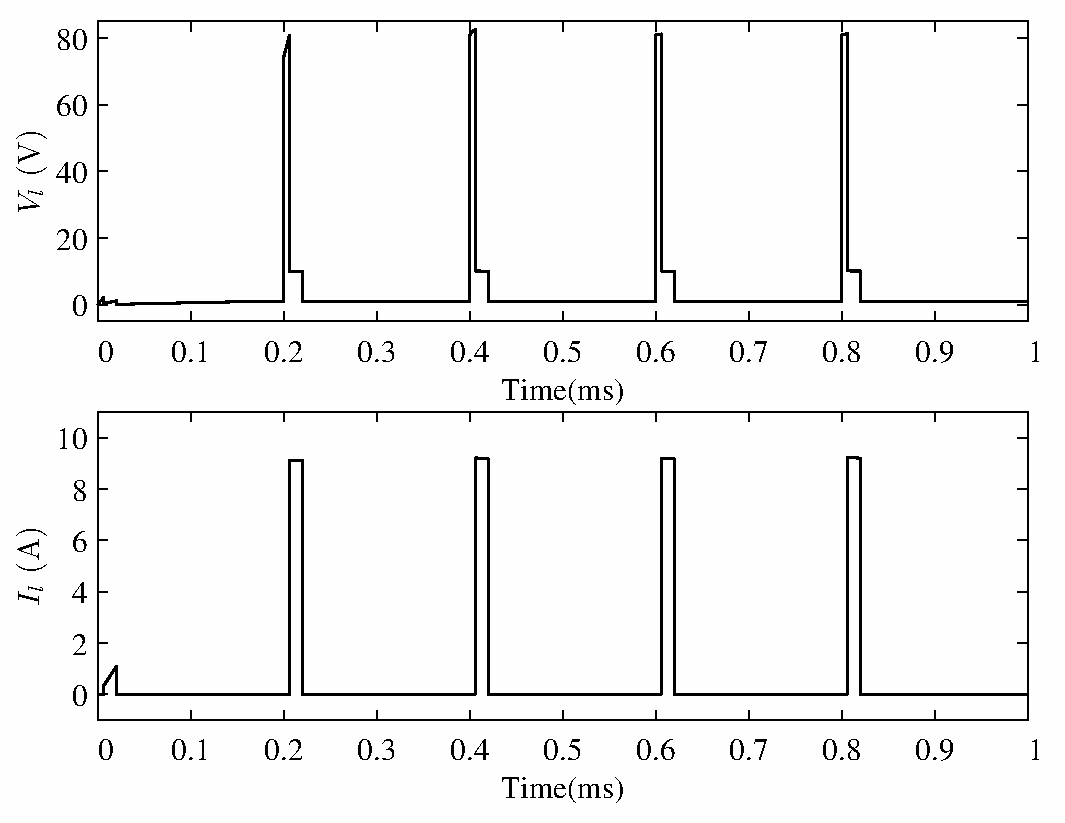
\includegraphics[width=0.8\textwidth]{load_cmc}
  \caption{Load voltage and current - current mode control}
  \label{fig:sim-cmc}
  \end{figure}
\end{frame}


\section{Practical Considerations}
\begin{frame}{Selection of inductors and capacitor}
\begin{enumerate}
\item Inductor for current source $\rightarrow$ Output current ripple
  \begin{equation}
    \Delta I_L = \dfrac{V_{o1}}{L_1} (1-D) T_s
    \label{eq:ind-1}
  \end{equation}
\item Inductor for voltage source $\rightarrow$ Maintaining continuous conduction mode
  \begin{equation}
    L_2 \geq 2.5\dfrac{DT_s}{I_{L_2}}(V_d-V_{\text{ref}})
    \label{eq:ind-4}
  \end{equation}
\item Capacitor for voltage source $\rightarrow$ Output voltage ripple
  \begin{equation}
    C_2 \geq \dfrac{\Delta I_{L_2}T_s}{8\Delta V_{o2}}
    \label{eq:ind-4a}
  \end{equation}
\end{enumerate}
\end{frame}
\begin{comment}
\begin{frame}{Snubber design of $Q_d$}

\end{frame}
\end{comment}
\begin{frame}{Required device ratings}
\begin{table}
  \begin{tabular}{l | l l l}
    \hline
    Device & $V_{\text{max}}$ & $I_{\text{max}}$ & $P_{\text{max}}$ \\
    \hline
    $Q_d$ & 80 V & 11 A & 880 W \\
    $D$ & 83 V & 0.8 A & 66.4 W \\
    $Q_1$ & 110 V & 11 A & 1210 W \\
    $D_1$ & 110 V & 11 A & 1210 W \\
    $Q_2$ & 110 V & 21 A & 2310 W \\
    $D_2$ & 110 V & 4.5 A & 495 W \\
    $Q_3$ & 110 V & 4.5 A & 495 W\\
    $D_1$ & 110 V & 21 A & 2310 W
  \end{tabular}
\end{table}
\end{frame}

\section{Summary and Future Plan}
\begin{frame}{Work Done}
\begin{itemize}
\item Power supply topology fixed
\item Converter modelled using time averaging
\item Controller designed using
\begin{itemize}
\item Direct duty ratio control \textendash{} PI controller, lead-lag compensator
\item Current mode control
\end{itemize}
\item Ratings passive components determined
\item Snubber circuit designed for $Q_d$
\item Simulated power supply
\item Approximate ratings of switches determined
\end{itemize}
\end{frame}
\begin{frame}{Future plan}
\textbf{Fabrication of Power Supply}
\begin{itemize}
\item Designing gate drivers
\item Designing and PCBs
\item Fabricating power supply
\item Testing of power supply \textendash{} metal, silicon
\end{itemize}
\textbf{Load Modelling}
\begin{itemize}
\item Electrical characterisation of spark gap load
\item Physical model R, L and C elements
\item Fitting mathematical model
\end{itemize}
\end{frame}


\begin{frame}[allowframebreaks]{References}
  \bibliography{../references/references}
  \bibliographystyle{IEEEtran}
\end{frame}

\appendix
\begin{frame}[allowframebreaks]{}
Small signal transfer function of voltage source
    \begin{multline}
    \dfrac{\hat{v}_o(s)}{\hat{d}(s)} = C[sI-A]^{-1}[(A_1-A_2)X+(B_1-B_2)V_d]+(C_1-C_2)X
    \label{eq:mod27a}
  \end{multline}

Small signal transfer function of current source
  \begin{multline}
    \dfrac{\hat{i}_o(s)}{\hat{d}(s)} = C[sI-A]^{-1}[(A_1-A_2)X+(B_1-B_2)V_d]+(C_1-C_2)X
    \label{eq:mod35}
  \end{multline}
\end{frame}

  \begin{figure}
    \centering
    \includesvg[width=0.7\textwidth]{expanded-no-ramp}
    \caption{Expanded view of perturbed inductor current}
    \label{fig:20}
  \end{figure}

  \begin{equation}
    i_L(nT_s) = i_L(0)\left( -\dfrac{D}{1-D} \right)^n
    \label{eq:7}
  \end{equation}

  \begin{figure}
    \centering
    \includesvg[width=0.7\textwidth]{expanded-ramp}
    \caption{Expanded view of inductor current with artificial ramp in presence of disturbance}
    \label{fig:23}
  \end{figure}

  \begin{equation}
    \hat{i}_L(nT_s) = \hat{i}_L(0)\left(-\dfrac{m_2-m_a}{m_1+m_a} \right)^n
    \label{eq:13}
  \end{equation}

  \begin{equation}
    \alpha = -\dfrac{1-\dfrac{m_a}{m_2}}{\dfrac{1-D}{D}+\dfrac{m_a}{m_2}}
    \label{eq:15}
  \end{equation}

\end{document}